\documentclass{oblivoir}
\usepackage{amsmath,amssymb,amsthm,kotex,paralist,kswrapfig}

\usepackage[skipabove=10pt,innertopmargin=10pt]{mdframed}

\usepackage{tabto,pifont}
\TabPositions{0.2\textwidth,0.4\textwidth,0.6\textwidth,0.8\textwidth}
\newcommand\tabb[5]{\par\bigskip\noindent\ding{172}\:{\ensuremath{#1}}
\tab\ding{173}\:\:{\ensuremath{#2}}\tab\ding{174}\:\:{\ensuremath{#3}}
\tab\ding{175}\:\:{\ensuremath{#4}}\tab\ding{176}\:\:{\ensuremath{#5}}}
\newcommand\tabfive[5]{\par\medskip\noindent\ding{172}\:\:{\ensuremath{#1}}\\
\ding{173}\:\:{\ensuremath{#2}}\\\ding{174}\:\:{\ensuremath{#3}}\\
\ding{175}\:\:{\ensuremath{#4}}\\\ding{176}\:\:{\ensuremath{#5}}}

\usepackage{enumitem}
\setlist[enumerate]{label=(\arabic*)}

\newcounter{num}
\newcommand{\defi}[1]
{\noindent\refstepcounter{num}\textbf{정의 \arabic{num}) #1}\par\noindent}
\newcommand{\theo}[1]
{\noindent\refstepcounter{num}\textbf{정리 \arabic{num}) #1}\par\noindent}
\newcommand{\exam}[1]
{\bigskip\bigskip\noindent\refstepcounter{num}\textbf{예시 \arabic{num}) #1}\par\noindent}
\newcommand{\prob}[1]
{\bigskip\bigskip\noindent\refstepcounter{num}\textbf{문제 \arabic{num}) #1}\par\noindent}
\newcommand{\proo}
{\bigskip\textsf{증명)}\par}

\newcommand{\ans}{
{\par
\raggedleft\textbf{답 : (\qquad\qquad\qquad\qquad\qquad\qquad)}
\par}\bigskip\bigskip}
\newcommand{\procedure}[1]{\begin{mdframed}\vspace{#1\textheight}\end{mdframed}}
\newcommand\an[1]{\par\bigskip\noindent\textbf{문제 #1)}\\}

\newcommand{\pb}[1]%\Phantom + fBox
{\fbox{\phantom{\ensuremath{#1}}}}
\newcommand\ba{\,|\,}

\let\oldsection\section
\renewcommand\section{\clearpage\oldsection}

\renewcommand{\arraystretch}{1.5}

\let\emph\textsf
%%%%
\begin{document}

\title{윤영 : 11 함수(2)}
\author{}
\date{\today}
\maketitle
\tableofcontents
\newpage

%%
\section{합성함수}
\kswrapfig[Pos=r,Width=5cm]{composition}{
세 집합 \(X\), \(Y\), \(Z\)에 대하여 두 함수
\begin{gather*}
f:X\to Y\\
g:Y\to Z
\end{gather*}
가 주어졌을 때, 집합 \(X\)의 각 원소 \(x\)들은 \(f\)에 의해 \(Y\)의 원소인 \(f(x)\)로 대응되고, \(f(x)\)는 다시 \(g\)에 의해 \(Z\)의 원소인 \(g(f(x))\)로 대응될 수 있다.}

\begin{mdframed}
%
\defi{합성함수}
이렇게 집합 \(X\)의 각각의 원소 \(x\)를 집합 \(Z\)의 원소 \(g(f(x))\)로 대응시켜 \(X\)를 정의역, \(Z\)를 공역으로 하는 새로운 함수를 정의할 수 있다.
이 함수를 \(f\)와 \(g\)의 \emph{합성함수}라고 하고, 이것을 기호로
\[g\circ f:X\to Z\]
로 나타낸다.
이때,
\[(g\circ f)(x)=g(f(x))\]
이다.
\end{mdframed}

%
\exam{}
\begin{enumerate}
\item
\(X=\{1,2,3\}\), \(Y=\{a,b,c,d\}\), \(Z=\{2,4,6\}\)일 때, 두 함수 \(f:X\to Y\), \(g:Y\to Z\)를
\begin{align*}
&f(1)=a 	&g(a)=6\\
&f(2)=c 	&g(b)=4\\
&f(3)=c 	&g(c)=2\\
&		&g(d)=2
\end{align*}
로 정의하자.
이를 그림으로 나타내면
\begin{figure}
\centering
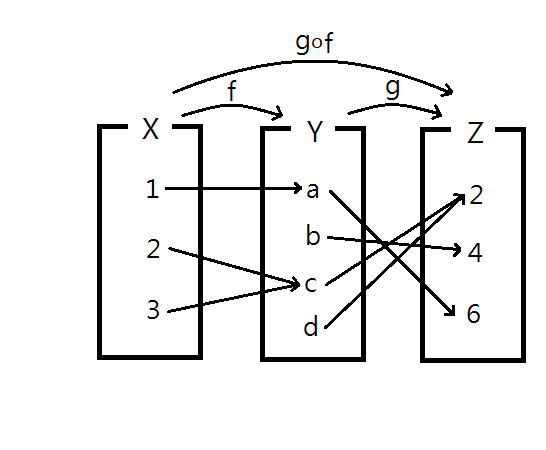
\includegraphics[width=0.5\textwidth]{composition_example}
\end{figure}

이므로
\begin{gather*}
(g\circ f)(1)=g(f(1))=g(a)=6\\
(g\circ f)(2)=g(f(2))=g(c)=2\\
(g\circ f)(3)=g(f(2))=g(c)=2
\end{gather*}
이다.
\item
두 함수 \(f(x)=x^2\), \(g(x)=2x\)에 대하여 \(g(2)=2\cdot 2=4\)이므로
\[(f\circ g)(2)=f(g(2))=f(4)=4^2=16\]
이다.
\end{enumerate}

\prob{}
두 함수 \(f(x)=x-1\)과 \(g(x)=-3x+8\)에 대하여 다음 함숫값을 구하여라.
\par\noindent
(1)\:\:\((f\circ g)(2)\)
\tabto{.5\textwidth}
(2)\:\:\((g\circ f)(-3)\)
\par\noindent
(3)\:\:\((f\circ f)(1)\)
\tabto{.5\textwidth}
(4)\:\:\((g\circ g)(0)\)

\clearpage
%
\exam{}\label{comm}
두 함수 \(f(x)=x+3\)과 \(g(x)=-2x-4\)에 대하여 다음을 구하여라.
\par\noindent
(1)\:\:\(f\circ g\)
\tabto{.5\textwidth}
(2)\:\:\(g\circ f\)
\begin{mdframed}
\begin{flalign*}
(1)\:\:(f\circ g)(x)
&=f(g(x))&\\
&=f(-2x-4)&\\
&=(-2x-4)+3&\\
&=-2x-1&\\
(2)\:\:(g\circ f)(x)
&=g(f(x))&\\
&=g(x+3)&\\
&=-2(x+3)-4&\\
&=-2x-10&
\end{flalign*}
\end{mdframed}
{\par\raggedleft\textbf{답 : (1) \((f\circ g)(x)=-2x-1\), (2) \((g\circ f)(x)=-2x-10\)}\par}\bigskip

\begin{mdframed}
%
\theo{}
예시 \ref{comm}에서 알 수 있듯이 일반적으로 두 함수 \(f\), \(g\)에 대하여
\[f\circ g\neq g\circ f\]
이다.
즉, 함수의 합성에 대하여 \emph{교환법칙}이 성립하지 않는다.
\end{mdframed}

%
\prob{}
두 함수 \(f(x)=x-2\), \(g(x)=x^2-4\)에 대하여 다음을 구하여라.
\par\noindent
(1)\:\:\(f\circ g\)
\tabto{.5\textwidth}
(2)\:\:\(g\circ f\)
\procedure{0.15}

%
\prob{}
두 함수 \(f(x)=2x+1\)과 \(g(x)=3x+a\)에 대하여 \(f\circ g=g\circ f\)가 되도록 실수 \(a\)의 값을 정하여라.
\procedure{0.3}

%
\exam{}\label{assoc}
세 함수 \(f(x)=4x\), \(g(x)=3x-1\), \(h(x)=2x\)에 대하여 다음을 구하여라.
\par\noindent
(1)\:\:\(h\circ(g\circ f)\)
\tabto{.5\textwidth}
(2)\:\:\((h\circ g)\circ f\)
\begin{mdframed}
\begin{enumerate}
\item
두 함수 \(f\), \(g\)의 합성함수 \(g\circ f\)는\\
\((g\circ f)(x)=g(f(x))=g(4x)=3\cdot4x-1=12x-1\)이므로
\[(h\circ(g\circ f))(x)=h((g\circ f)(x))=h(12x-1)=24x-2\]
\item
두 함수 \(g\), \(h\)의 합성함수 \(h\circ g\)는\\
\((h\circ g)(x)=h(g(x))=h(3x-1)=2(3x-1)=6x-2\)이므로
\[((h\circ g)\circ f)(x)=(h\circ g)(f(x))=(h\circ g)(4x)=24x-2\]
\end{enumerate}
\end{mdframed}
{\par\raggedleft\textbf{답 : 
(1) \((h\circ(g\circ f))(x)=24x-2\), 
(2) \(((h\circ g)\circ f)(x)=24x-2\)}\par}\bigskip

\begin{mdframed}
%
\theo{}
예시 \ref{assoc}에서 알 수 있듯이 일반적으로 세 함수 \(f\), \(g\), \(f\)에 대하여
\[h\circ(g\circ f)=(h\circ g)\circ f\]
이다.
즉, 함수의 합성에 대하여 \emph{결합법칙}이 성립한다.
\end{mdframed}

%
\prob{}
두 함수 \(f(x)=2x\), \(g(x)=x-1\), \(h(x)=x^2\)에 대하여 \(h\circ(g\circ f)=(h\circ g)\circ f\)임을 보여라.
\procedure{0.2}

%
\prob{}
함수 \(f(x)=x-3\)에 대하여 \((f\circ f\circ f)(0)+(f\circ f)(18)\)의 값을 구하여라.
\procedure{0.2}

\clearpage
%
\theo{}
함수 \(f:X\to Y\)와 항등함수 \(I\)를 생각하자.
즉
\[I(x)=x\]
이다.
이때 \(f\circ I\)와 \(I\circ f\)를 각각 계산해보면
\begin{gather*}
(f\circ I)(x)=f(I(x))=f(x)\\
(I\circ f)(x)=I(f(x))=f(x)
\end{gather*}
이다.
따라서 
\begin{mdframed}[skipabove=5pt,skipbelow=5pt,leftmargin=120pt,rightmargin=120pt]
\[f\circ I=I\circ f=f\]
\end{mdframed}
이다.

\(f\circ I\)에서의 \(I\)는 정의역과 공역이 \(X\)인 항등함수인 \(I_X\)이고, \(I\circ f\)에서의 \(I\)는 정의역과 공역이 \(Y\)인 항등함수인 \(I_Y\)이다.
그러므로 위의 식을 더 정확히 쓰면
\begin{mdframed}[skipabove=5pt,skipbelow=5pt,leftmargin=120pt,rightmargin=120pt]
\[f\circ I_X=I_Y\circ f=f\]
\end{mdframed}
가 된다.

%\bigskip
%\(f\)와 \(I\)를 합성하면 \(f\)가 된다.
%다시 말해, \(I\)는 합성하여도 아무 역할을 못한다.
%이러한 \(I\)는 덧셈에서의 0, 곱셈에서의 1과 비슷한 성질을 가진다.
%\begin{align*}
%a+0=0+a=a\\
%a\times1=1\times a=a\\
%f\circ I=I\circ f=f
%\end{align*}

%%
\section{역함수}
세 함수 \(f\), \(g\), \(h\)에서, 반대 방향의 대응이 집합 \(Y\)에서 집합 \(X\)로의 함수가 되는지 알아보자.
\begin{figure*}[h!]
\centering
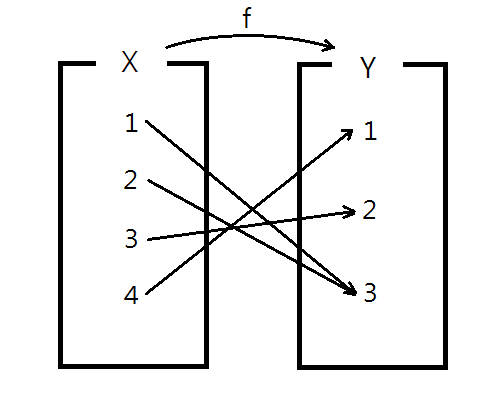
\includegraphics[width=0.3\textwidth]{inverse_1}
~
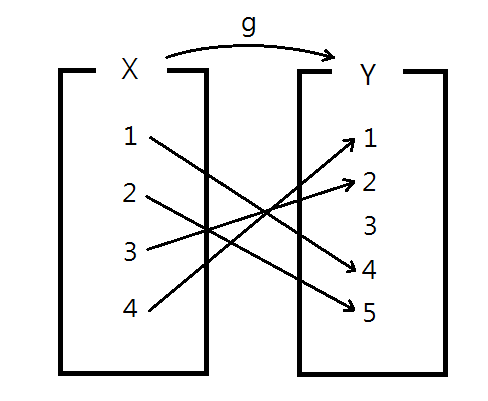
\includegraphics[width=0.3\textwidth]{inverse_2}
~
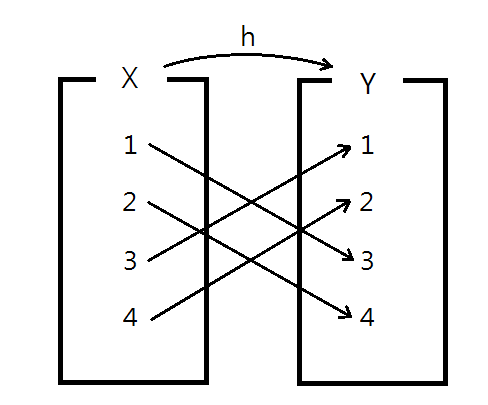
\includegraphics[width=0.3\textwidth]{inverse_3}
\end{figure*}
\begin{enumerate}
\item
함수 \(f\)의 경우에는 \(Y\)의 원소 \(3\)에 대응하는 \(X\)의 원소가 두 개이므로, 함수 \(f\)의 반대방향의 대응은 함수가 아니다.
\item
함수 \(g\)의 경우에는 \(Y\)의 원소 \(3\)에 대응하는 \(X\)의 원소가 없으므로, 함수 \(g\)의 반대방향의 대응도 함수가 아니다.
\item
함수 \(h\)의 경우에는 \(Y\)의 각 원소에 \(X\)의 원소가 하나씩 대응하므로 함수 \(h\)의 반대방향의 대응은 함수이다.
\end{enumerate}
이때, \(f\)는 일대일 함수가 아니고 따라서 일대일 대응도 아니다.
\(g\)는 일대일 함수이지만 일대일 대응은 아니다.
반면 \(h\)는 일대일 대응이다.

\begin{mdframed}
%
\defi{역함수}
함수 \(f:X\to Y\)가 일대일 대응일 때, 집합 \(Y\)의 각 원소 \(y\)에 \(y=f(x)\)를 만족시키는 집합 \(X\)의 원소 \(x\)를 대응시켜 \(Y\)를 정의역, \(X\)를 공역으로 하는 새로운 함수를 정의할 수 있다.
이 함수를 \(f\)의 \emph{역함수}라고 하며, 이것을 기호로
\[f^{-1}:Y\to X\]
로 나타낸다.
또
\[x=f^{-1}(y)\]
라고 쓴다.
\end{mdframed}

\clearpage
\begin{figure}[h!]
\center
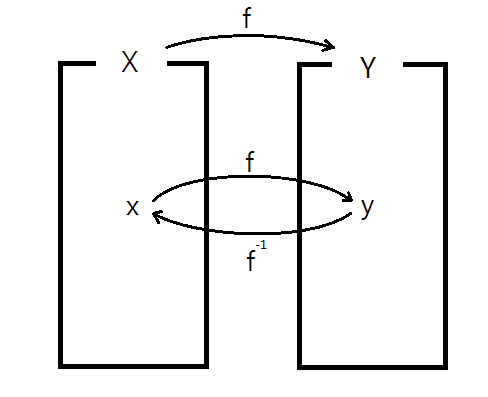
\includegraphics[width=0.4\textwidth]{inverse_xy}
\end{figure}

\vspace{-20pt}
%
\prob{}
다음 함수 중 역함수가 존재하는 함수를 모두 말하여라.
\begin{figure}[h!]
\centering\noindent
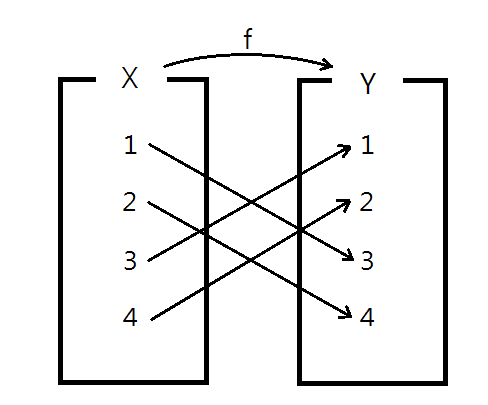
\includegraphics[width=0.35\textwidth]{inverse_example_1}
~
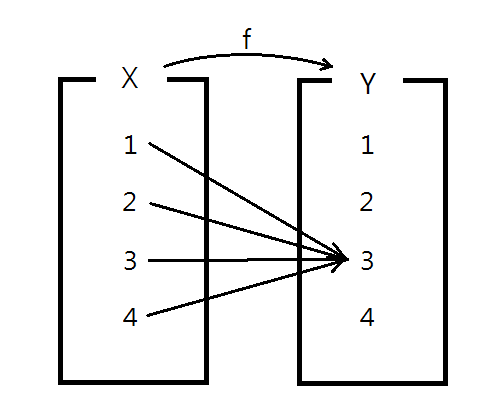
\includegraphics[width=0.35\textwidth]{inverse_example_2}
\par\noindent(1)\qquad\qquad\qquad\qquad\qquad\qquad\qquad(2)\par\noindent
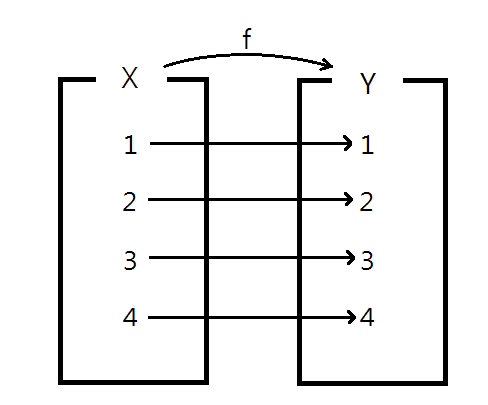
\includegraphics[width=0.35\textwidth]{inverse_example_3}
~
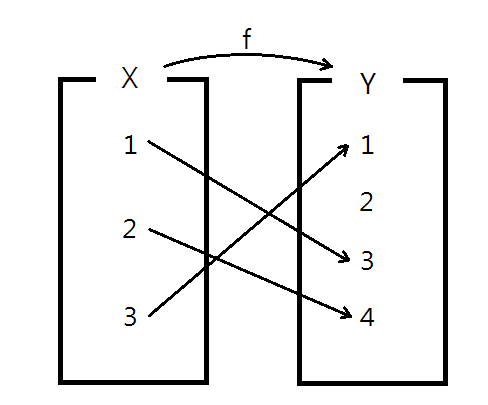
\includegraphics[width=0.35\textwidth]{inverse_example_4}
\par\noindent(3)\qquad\qquad\qquad\qquad\qquad\qquad\qquad(4)
\end{figure}

\kswrapfig[Pos=r,Width=5cm]{inverse_example_5}{
\setcounter{num}{14}
%
\prob{}
함수 \(f:X\to Y\)의 역함수가 존재하도록 오른쪽 그림을 완성하고 다음을 구하여라.
\begin{enumerate}
\item
\(f(5)+f^{-1}(5)\)
\item
\(f^{-1}(a)=2\)를 만족하는 상수 \(a\)의 값
\end{enumerate}}

\begin{mdframed}
%
\theo{역함수의 성질}\label{property}
함수 \(f:X\to Y\)가 일대일 대응일 때
\begin{enumerate}
\item
역함수 \(f^{-1}:Y\to X\)가 존재한다.
\item
\(y=f(x)\quad\iff\quad x=f^{-1}(y)\)
\item
\((f^{-1})^{-1}(x)=f(x)\) (\(x\in X\))
\item
\((f^{-1}\circ f)(x)=x\) (\(x\in X\)),\quad \((f\circ f^{-1})(y)=y\) (\(y\in Y\))
\end{enumerate}
\end{mdframed}
\proo
(1)은 당연하다.
함수 \(f:X\to Y\)의 역함수가 존재할 때 \(x\in X\)와 \(y\in Y\)에 대하여
\[y=f(x)\quad\iff\quad x=f^{-1}(y)\]
이다.
따라서 (2)가 성립한다.
\(x=f^{-1}(y)\)에 (2)를 한 번 더 쓰면 \(y=(f^{-1})^{-1}(x)\)인데, \(y=f(x)\)이므로
\[(f^{-1})^{-1}(x)=f(x)\]
이다.
따라서 (3)이 성립하며, (3)은
\begin{mdframed}[skipabove=5pt,skipbelow=5pt,leftmargin=120pt,rightmargin=120pt]
\[(f^{-1})^{-1}=f\]
\end{mdframed}
로 쓸 수도 있다.
또
\begin{align*}
(f^{-1}\circ f)(x)&=f^{-1}(f(x))=f^{-1}(y)=x\\
(f\circ f^{-1})(y)&=f(f^{-1}(y))=f(x)=y
\end{align*}
이다.
따라서 (4)가 성립하며, (4)는
\begin{mdframed}[skipabove=5pt,skipbelow=5pt,leftmargin=120pt,rightmargin=120pt,innertopmargin=0pt]
\begin{gather*}
f^{-1}\circ f=I_X\\
f\circ f^{-1}=I_Y
\end{gather*}
\end{mdframed}
로 쓸 수도 있다.

\clearpage
\kswrapfig[Pos=r,Width=4cm]{inverse_example_6}{
%
\exam{}
오른쪽 그림의 함수 \(f:X\to Y\)에 대하여 다음을 구하여라.
\par\noindent
(1)\:\:\(f^{-1}(b)\)
\tabto{.5\textwidth}
(2)\:\:\((f\circ f^{-1})(a)\)}
\begin{mdframed}
\begin{enumerate}
\item
\(f^{-1}(b)\)는 역함수 \(f^{-1}\)에 의한 \(b\)의 함숫값이므로 \(b\)에서 반대 화살표를 따라가서 얻을 수 있는 \(1\)이다.
즉 \(f^{-1}(b)=1\)이다.

\textbf{(다른방법)}
\(f^{-1}(b)=k\)라고 두면 정리 \ref{property}의 (2)에 의해 \(f(k)=b\)이다.
\(f(k)=b\)인 \(k\)는 \(1\)이므로 \(k=1\)이다.
즉 \(f^{-1}(b)=1\)이다.
\item
\((f\circ f^{-1})(a)=f(f^{-1}(a))=f(2)=a\)이다.

\textbf{(다른방법)}
\(f\circ f^{-1}=I\)이므로 \((f\circ f^{-1})(a)=I(a)=a\)이다.
\end{enumerate}
\end{mdframed}

\kswrapfig[Pos=r,Width=4cm]{inverse_example_7}{%
\prob{}
오른쪽 그림의 함수 \(f:X\to Y\)에 대하여 다음을 구하여라.
\par\noindent
(1)\:\:\(f^{-1}(a)\)
\tabto{.35\textwidth}
(2)\:\:\((f^{-1})^{-1}(4)\)
\par\noindent
(3)\:\:\((f^{-1}\circ f)(3)\)
\tabto{.35\textwidth}
(4)\:\:\((f\circ f^{-1})(b)\)}
\procedure{0.35}

함수 \(y=f(x)\)에서 \(y=f(x)\)와 동치인 식은
\[x=f^{-1}(y)\]
이다.
여기에 \(x\)와 \(y\)를 서로 바꾸면
\[y=f^{-1}(x)\]
이다.

\begin{mdframed}
\begin{center}
역함수를 구한다.
\(\qquad\Rightarrow\qquad\)
\(x\)와 \(y\)를 서로 바꾸어 \(y\)에 관해 정리한다.
\end{center}
\end{mdframed}

%
\exam{}
함수 \(y=4x+3\)의 역함수를 구하여라.
\begin{mdframed}
\(x\)와 \(y\)를 바꾸면
\[x=4y+3\]
이 되고 이것을 다시 \(y\)에 대해 정리하면
\[y=\frac14x-\frac34\]
이다.
따라서 구하는 역함수는 \(y=\frac14x-\frac34\)이다.
\end{mdframed}

%
\prob{}
다음 함수의 역함수를 구하여라.
\par\noindent
(1)\:\:\(y=-3x+3\)
\tabto{.5\textwidth}
(2)\:\:\(y=\frac14x+1\)
\procedure{0.2}

수학 1에서 대칭이동에 관해 배울 때, \(x\)와 \(y\)를 서로 바꾼 식의 그래프는 원래 식의 그래프와 직선 \(y=x\)에 대해 대칭이라고 했다.

\kswrapfig[Pos=r]{y=x_transform}{
예를 들어, 원
\[(x-2)^2+y^2=1\]
에서 \(x\)와 \(y\)를 서로 바꾸면 
\[x^2+(y-2)^2=1\]
이 되는데
원래 식의 그래프와 바꾼 식의 그래프를 비교하면 두 원은 \(y=x\)에 대해 대칭이다.}

\bigskip\medskip
함수 \(y=f(x)\)에서 \(x\)와 \(y\)를 서로 바꾸면 \(y=f^{-1}(x)\)가 되므로 다음이 성립한다.
\begin{mdframed}
%
\theo{}
함수 \(y=f(x)\)의 그래프와 그 역함수 \(y=f^{-1}(x)\)의 그래프는 직선 \(y=x\)에 대하여 대칭이다.
\end{mdframed}

%
\exam{}
함수 \(y=2x+1\)의 역함수는 \(y=\frac12x-\frac12\)
이므로 두 함수의 그래프를 그리면 아래
그림과 같다.
이 그림으로부터 함수 \(y=2x+1\)의 그래프와 \(y=\frac12x-\frac12\)의 그래프는 직선 \(y=x\)에 대하여 서로 대칭임을 알 수 있다.
\begin{figure*}[h!]
\centering
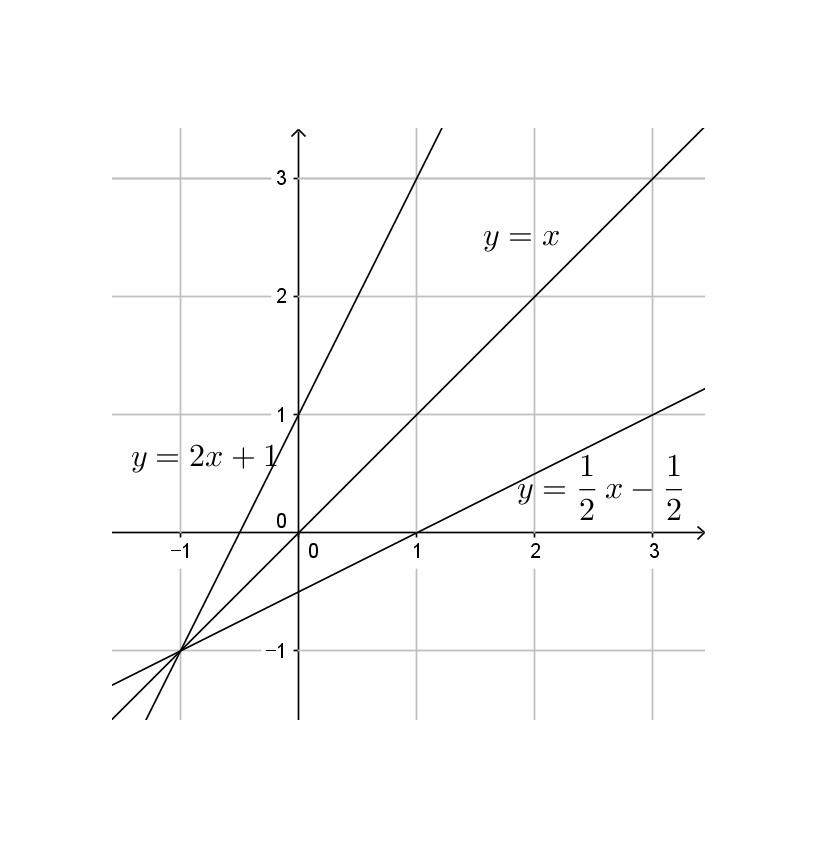
\includegraphics[width=0.4\textwidth]{y=2x+1}
\end{figure*}

%
\prob{}
다음 함수와 그 역함수의 그래프를 좌표평면 위에 그려라.
\par\noindent
(1)\:\:\(y=x+1\)
\tabto{.5\textwidth}
(2)\:\:\(y=2x-2\)
\begin{figure*}[h!]
\centering\noindent
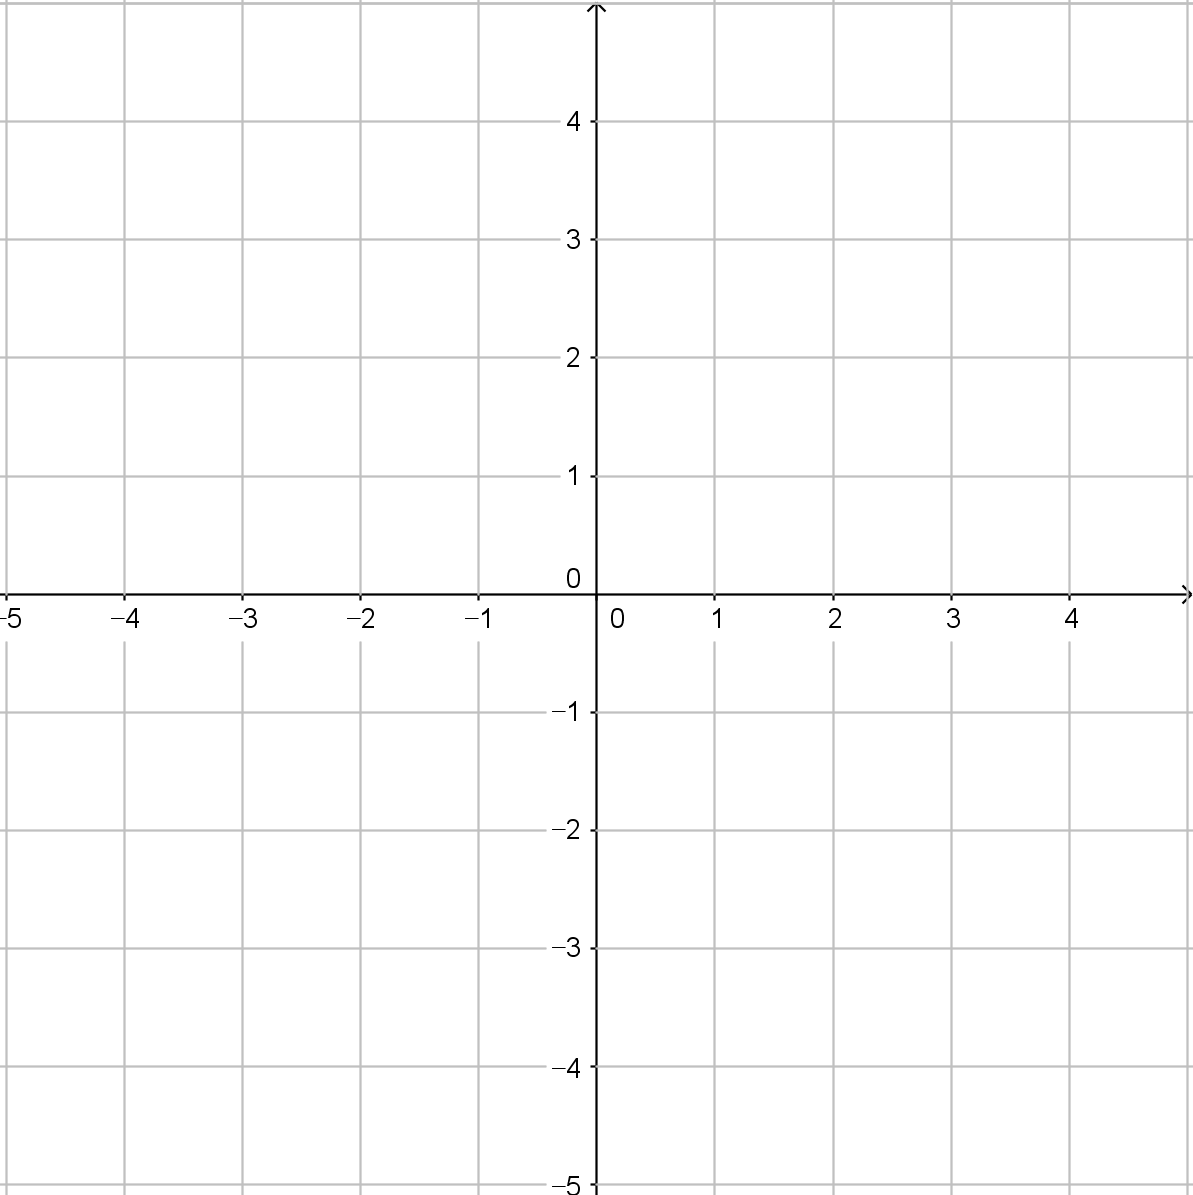
\includegraphics[width=0.4\textwidth]{pm4by4}
\hspace{50pt}
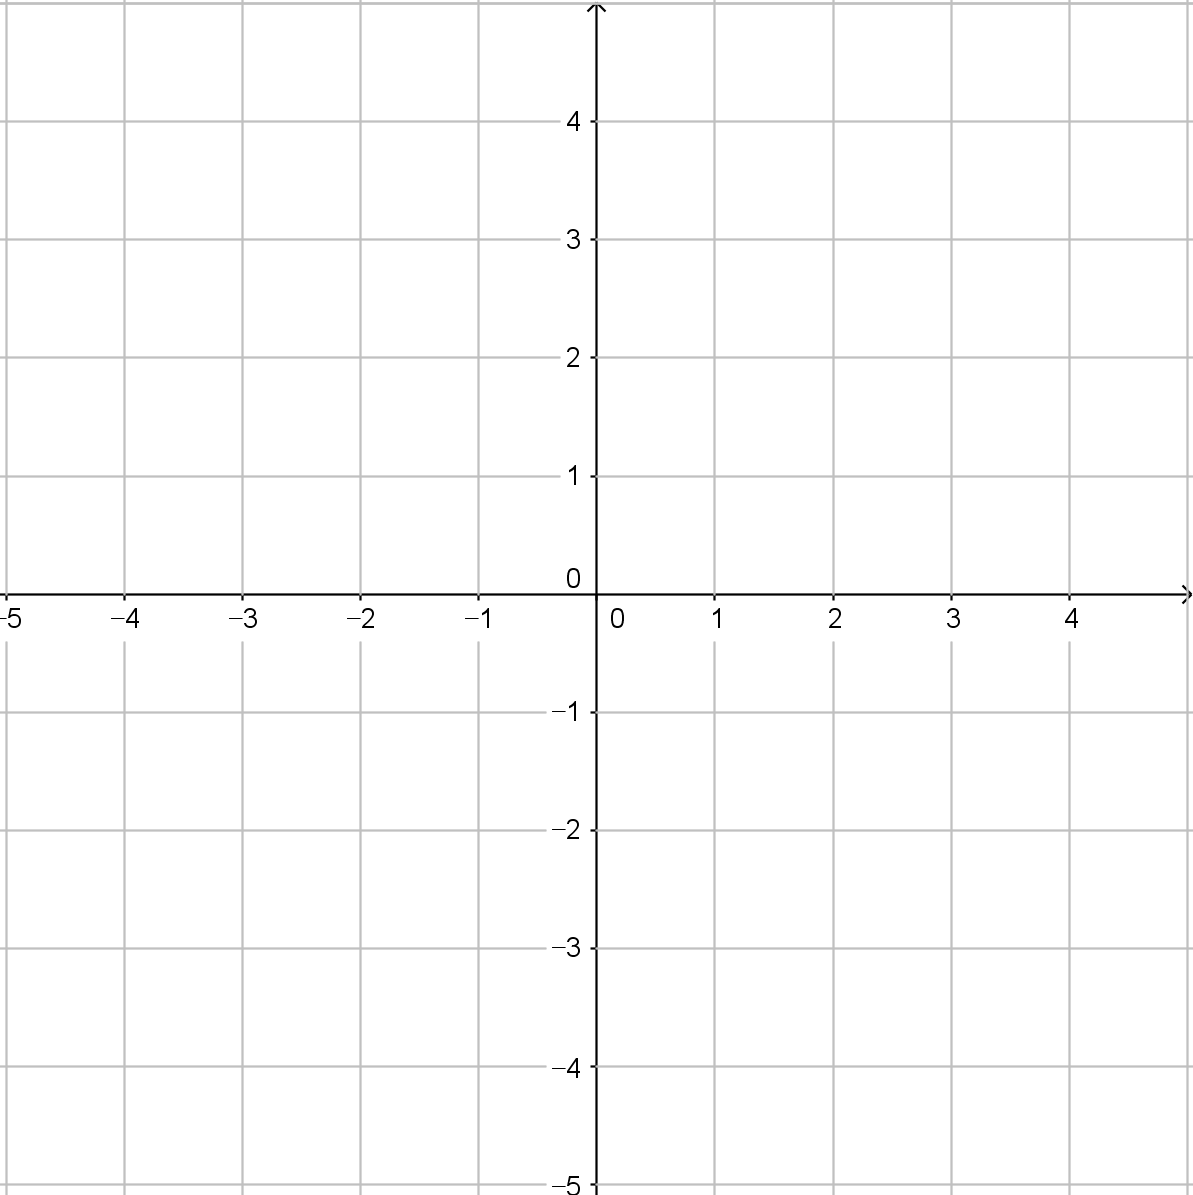
\includegraphics[width=0.4\textwidth]{pm4by4}
\end{figure*}

%
\prob{}
두 함수 \(f(x)=x+3\), \(g(x)=3x-4\)에 대하여 다음 물음에 답하여라.
\begin{enumerate}
\item
두 역함수 \(f^{-1}(x)\), \(g^{-1}(x)\)를 구하여라.
\item
합성함수 \((g\circ f)(x)\)와 그 역함수 \((g\circ f)^{-1}(x)\)를 구하여라.
\item
\((f^{-1}\circ g^{-1})(x)를 구하여라.\)
\procedure{0.3}

\begin{mdframed}
%
\theo{}
일대일 대응인 두 함수 \(f\), \(g\)의 합성함수 \(g\circ f\)가 존재하면
\[(g\circ f)^{-1}(x)=f^{-1}\circ g^{-1}\]
이다.
\end{mdframed}
\end{enumerate}

%%
\section{보충 · 심화 문제}
%
\prob{}
\(A\) 상점과 \(B\) 상점은 모든 제품을 다음과 같이 할인하여 판매하고 있다.
\begin{mdframed}[skipbelow=10pt]
\(A\) 상점 : 정가의 \(5\)\%를 할인한 후 \(5000\)원을 추가로 할인.\\
\(B\) 상점 : 정가에 \(5000\)원을 할인한 후 \(5\)\%를 추가로 할인.
\end{mdframed}
정가가 동일한 상품을 구매하려고 할 때, 어느 상점에서 구매하는 것이 구매자에게 유리한가?
\vspace{0.25\textheight}

%
\prob{}
두 집합 \(X=\{x\ba0\le x\le 2\}\), \(Y=\{y\ba0\le y\le a\}\)에 대하여\\
함수 \(f:X\to Y\), \(y=bx+1\) (\(b<0\))일 때, 역함수 \(f^{-1}:Y\to X\)가 존재하도록 두 실수 \(a\), \(b\)의 값을 정하여라.
\vspace{0.35\textheight}

%
\prob{}
집합 \(X=\{1,2,3,4\}\)에 대하여 함수 \(f\)가 오른쪽 그림과 같을 때, 다음 값을 구하여라.
\par\noindent
(1)\:\:\((f\circ f)(2)\)
\tabto{.5\textwidth}
(2)\:\:\((f\circ f\circ f)(3)\)
\vspace{0.1\textheight}

%
\prob{}
함수 \(f(x)=x-1\)에 대하여
\[f_1(x)=f(x),\quad f_{n+1}(x)=(f\circ f_n)(x)\:\:(n\text{은 자연수})\]
로 정의할 때, \(f_{30}(2)\)의 값을 구하여라.
\vspace{0.1\textheight}

%
\prob{}
실수 전체의 집합에서 정의된 두 함수 \(f(x)=3x-4\), \(g(x)=x+6\)에 대하여 합성함수 \(h(x)=(f\circ(g\circ f)^{-1}\circ f)(x)\)일 때, \(h(3)+h^{-1}(2)\)의 값을 구하여라.
\vspace{0.1\textheight}

%%
\section*{답}

\begin{minipage}{0.49\textwidth}
%
\an{3}
\begin{enumerate}[topsep=0pt]
\item
\(1\)
\item
\(20\)
\item
\(-1\)
\item
\(-16\)
\end{enumerate}

%
\an{6}
\begin{enumerate}[topsep=0pt]
\item
\((f\circ g)(x)=x^2-6\)
\item
\((g\circ f)(x)=x^2-4x\)
\end{enumerate}

%
\an{7}
\(2\)

%
\an{10}
\begin{enumerate}[topsep=0pt]
\item
두 함수 \(f\), \(g\)의 합성함수 \(g\circ f\)는\\
\((g\circ f)(x)=g(f(x))=g(2x)=2x-1\)이므로
\begin{align*}
(h\circ(g\circ f))(x)
&=h((g\circ f)(x))\\
&=h(2x-1)=4x^2-4x+1
\end{align*}
\item
두 함수 \(g\), \(h\)의 합성함수 \(h\circ g\)는\\
\((h\circ g)(x)=h(g(x))=h(x-1)=(x-1)^2=x^2-2x+1\)이므로
\begin{align*}
((h\circ g)\circ f)(x)
&=(h\circ g)(f(x))\\
&=(h\circ g)(2x)=4x^2-4x+1
\end{align*}
\end{enumerate}
\end{minipage}
%%%
\begin{minipage}{0.49\textwidth}
따라서 \(h\circ(g\circ f)=(h\circ g)\circ f\)이다.

%
\an{11}
\(3\)

%
\an{14}
(1), (3)

%
\an{15}
(그림생략), (1) \(7\), (2) \(9\)

%
\an{19}
\begin{enumerate}[topsep=0pt]
\item
\(3\)
\item
\(c\)
\item
\(3\)
\item
\(b\)
\end{enumerate}

%
\an{21}
\begin{enumerate}[topsep=0pt]
\item
\(y=-\frac13x+1\)
\item
\(y=4x-4\)
\end{enumerate}
\end{minipage}

\begin{minipage}{0.49\textwidth}
%
\an{24}
\begin{center}
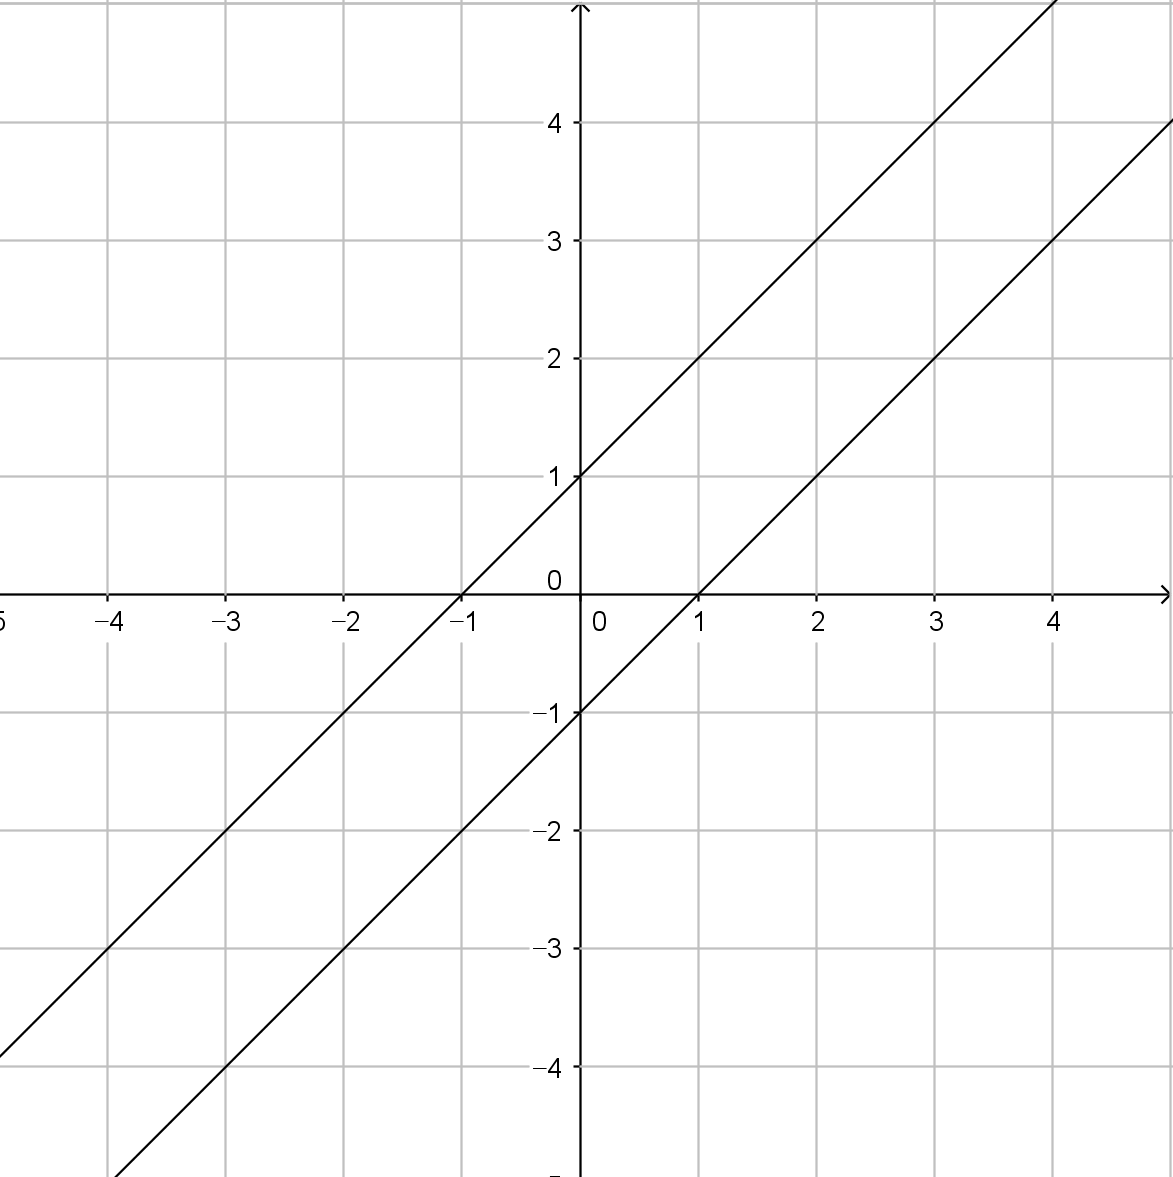
\includegraphics[width=0.45\textwidth]{y=x+1}
~
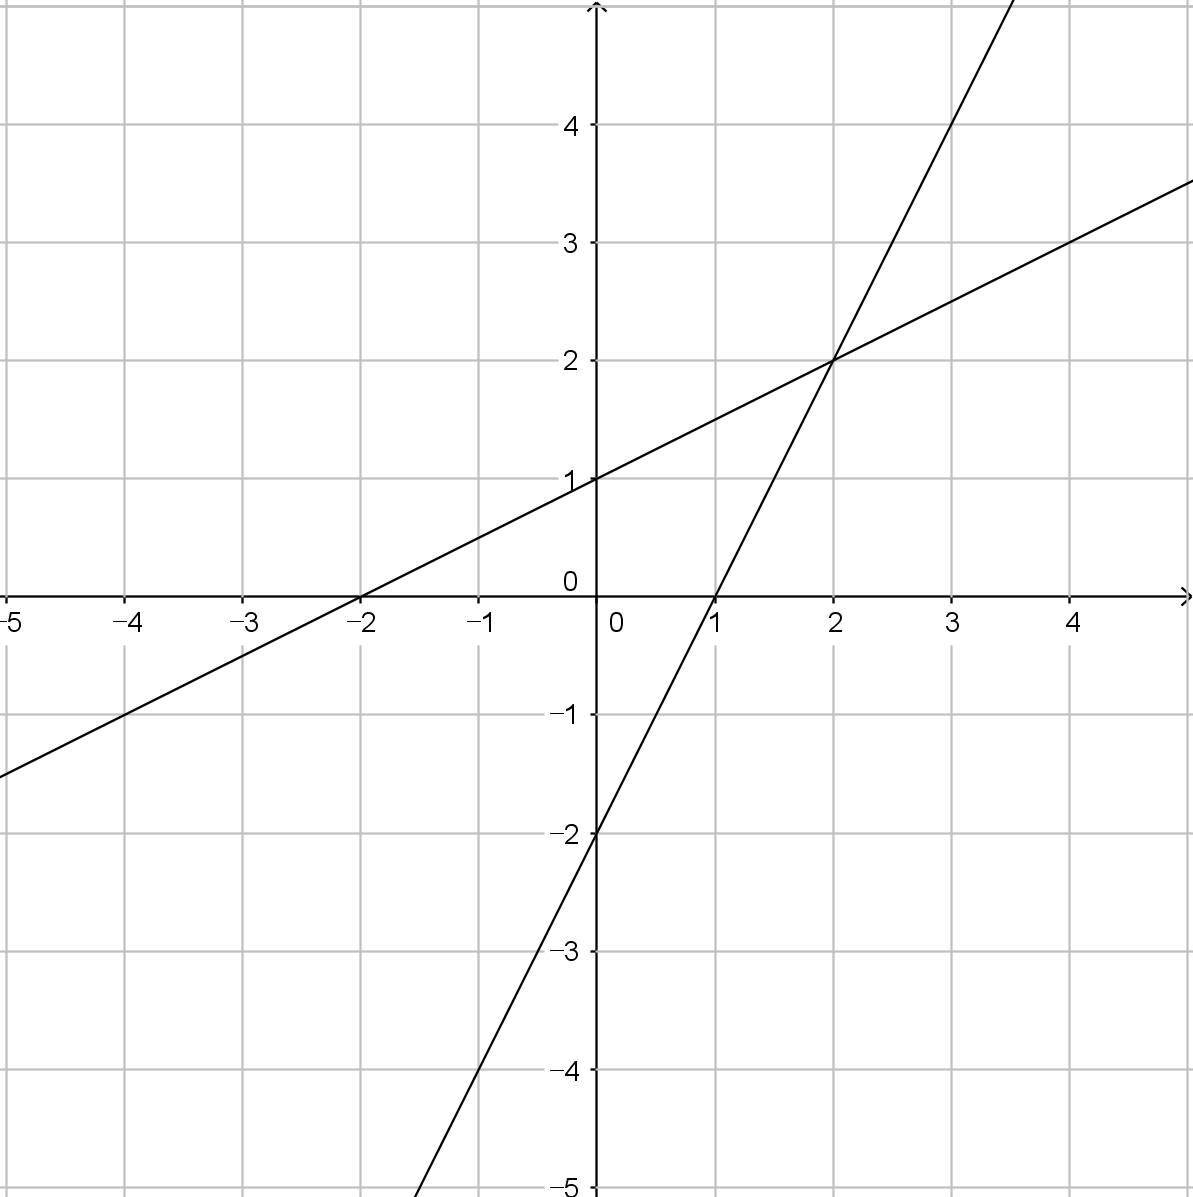
\includegraphics[width=0.45\textwidth]{y=2x-2}
\par\noindent(1)\qquad\qquad\qquad\quad\:\:(2)
\end{center}

%
\an{25}
\begin{enumerate}[topsep=0pt]
\item
\(f^{-1}(x)=x-3\), \(g^{-1}(x)=\frac13x+\frac43\)
\item
\((g\circ f)(x)=3x+5\)\\
\((g\circ f)^{-1}(x)=\frac13x-\frac53\)
\item
\((f^{-1}\circ g^{-1})(x)=\frac13x-\frac53\)
\end{enumerate}
%
\an{27}
\(A\)상점이 더 유리하다.

%
\an{28}
\(a=1\), \(b=-\frac12\)

%
\an{29}
(1) 1, (2) 3

%
\an{30}
\(-28\)

%
\an{31}
\(3\)
\end{minipage}
\end{document}